\subparagraph{Shannon entropy $H_S(X)$} A concrete realization of an information entropy is given by the Shannon entropy
\begin{equation*}
	H_S=-\sum\limits_i P(x_i)\log_2(P(x_i))=-k_S\sum\limits_iP(x_i)\ln(P(x_i)) \qquad k_S=\ln(2)
\end{equation*}
The Shannon entropy measures entropy in bits. If we consider a random variable $X$ with possible values $X_i$ where $i=1,2,\ldots ,\Omega$, $p_i=P(x_i)$ and $\sum\limits_{i=1}^\Omega p_i=1$.\\
\underline{Properties}:
\begin{enumerate}[label={$(\arabic*)$}]
	\item \underline{Entropy is maximum for equal probabilities}
	\begin{equation*}
		H_I\left(\frac{1}{\Omega},\ldots,\frac{1}{\Omega}\right)>H_I(p_1,\ldots,p_\Omega) \quad \text{unless } p_i=\frac{1}{\Omega}\forall\ i
	\end{equation*}
	We note that $\mathcal{S}(p)=-p\ln(p)$ is concave in $]0,1[$, since $\mathcal{S}''(p)=-\frac{1}{p}<0$\\
\begin{figure}[H]
\begin{multicols}{2}
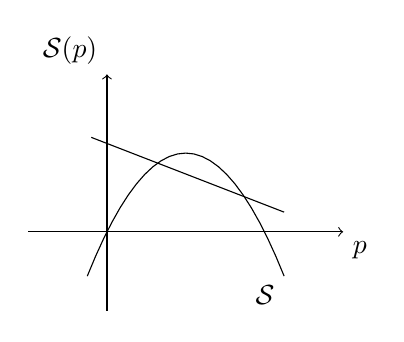
\begin{tikzpicture}
\draw[->] (-1,0)--(3,0)node[below right]{$p$};
\draw[->] (0,-1)--(0,2)node[above left]{$\mathcal{S}(p)$};
\draw (-0.2,1.2)--(2.25,0.25);
\draw[domain=-0.25:2.25] plot(\x,{-\x*(\x-2)})node[below left]{$\mathcal{S}$};
\end{tikzpicture}\\\columnbreak
\begin{align*}
x&=\lambda a+(1-\lambda b) \qquad \lambda\in ]0,1[\\
\to f(x)&=\mathcal{S}(\lambda a+(1-\lambda)b) > \lambda \mathcal{S}(a)+(1-\lambda)\mathcal{S}(b)
\end{align*}
\end{multicols}
\end{figure}
For a concave function, we get:
\begin{equation*}
\frac{1}{\Omega}\sum\limits_k\mathcal{S}(p_k)\leq \mathcal{S}\left(\frac{1}{\Omega}\sum\limits_kp_k\right)
\end{equation*}
This property can be shown by induction. For $\Omega=2$ we use $\lambda=\frac{1}{2}$, $a=p$ and $b=p_2\qquad \leadsto\ \mathcal{S}(\frac{p_1+p_2}{2})\geq\frac{1}{2}\left(\mathcal{S}(p_1)+\mathcal{S}(p_2)\right)$\\
For general $\Omega$ we use $\lambda=\frac{\Omega -1}{\Omega},\ a=\sum\limits_{k=1}^{\Omega -1}\frac{p_k}{\Omega -1}$ and $b=p_\Omega$
\begin{align*}
\mathcal{S}\left(\frac{\sum\limits_{k=1}^\Omega p_k}{\Omega}\right)&=\mathcal{S}\left(\frac{\Omega -1}{\Omega}\frac{\sum\limits_{i=1}^{\Omega -1}p_k}{\Omega -1}+\frac{1}{\Omega}p_\Omega\right)\\
&\geq \frac{\Omega -1}{\Omega}\mathcal{S}\left(\frac{\sum\limits_{k=1}^{\Omega -1} p_k}{\Omega -1}\right)+\frac{1}{\Omega}\mathcal{S}(p_\Omega)\\
&\geq \frac{\Omega -1}{\Omega}\frac{1}{\Omega -1}\sum\limits_{k=1}^{\Omega -1}\mathcal{S}(p_k)+\frac{1}{\Omega}\mathcal{S}(p_\Omega)=\frac{1}{\Omega}\sum\limits_{k=1}^\Omega\mathcal{S}(p_k)
\end{align*}
The identity leads to:
\begin{align*}
H_S(p_1,\ldots,p_\Omega)&=-\sum\limits_{k=1}^\Omega p_k\log_2(p_k)=\sum\mathcal{S}(p_k)\\
&\leq\Omega\mathcal{S}\left(\frac{1}{\Omega}\sum\limits_kp_k\right)=\Omega\mathcal{S}\left(\frac{1}{\Omega}\right)=-\sum\limits_{k=1}^\Omega\frac{1}{\Omega}\log_2\left(\frac{1}{\Omega}\right)\\
&=H_S\left(\frac{1}{\Omega},\ldots,\frac{1}{\Omega}\right)
\end{align*}
\item Entropy has the property that
\begin{equation*}
H_I(p_1,\ldots,p_{\Omega -1},0)=H_I(p_1,\ldots,p_{\Omega-1})
\end{equation*}
i.e. it does not change if we add states with probability 0.\\
This property is given, since $p\ln(p)\underset{p\to 0}{=}0$.
\item \underline{\smash{Entropy changes for conditional probabilities}}\\
We know that $P(A_k,B_l)$, i.e. the probability to find $A_k$ \textbf{and} $B_l$, can be expressed as $P(B_l)P(A_k|B_l)=P(A_k)P(B_l|A_k)=P(A_k,B_l)$ where $P(A_k|B_l)$ denotes the probability to find $A_k$ given that we have $B_l$. Obviously $P(A_k|B_l)=\frac{P(A_k,B_l)}{P(B_l)}$.\\
Conditional probabilities are normalized, i.e. we have
\begin{equation*}
\sum\limits_k P(A_k|B_l)=1
\end{equation*}
We now consider conditional probabilities for our ignorance function.\\
If we have $H_I(A)=H_I(p_1,\ldots,p_\Omega);\ H_I(B)=H_I(q_1,\ldots,q_\mu)$ for the two sets of states.\\
Then the ignorance function for the combined state space is given by
\begin{align*}
H_I(AB)&=H(r_{11},r_{12},\ldots,r_{\Omega\mu})\\
&=H(c_{11}q_1,c_{12}q_2,\ldots,c_{\Omega\mu}q_\mu)
\end{align*}
where $r_{ij}=P(A_i,B_j);\ q_i=P(B_i);\ c_{ij}=P(A_i|B_j)$\\
If we now select a state $q_l$ for our ignorance function, we get:
\begin{equation*}
H_I(A|B_l)=H_i(c_{1l},\ldots,c_{\Omega l})
\end{equation*}
What is the amount of information we typically gain by selecting $q_l$?
\begin{align*}
\langle H_I(A|B_l)\rangle=\sum\limits_lq_l\mathcal{S}_I(A|B_l)
\end{align*}
i.e. the average of the joint ignorance function.\\
For a proper ignorance function we would expect that:
\begin{equation*}
\langle H_I(A|B_l)\rangle=H(A,B)-H_I(B)
\end{equation*}
\begin{align*}
H_S(A,B)&=-k_s\sum\limits_{kl}c_{kl}q_l\ln(c_{kl}q_l) \qquad P_{kl}=P(A_k,B_l)=c_{kl}q_l\\
&=-k_S\left(\sum\limits_{kl}q_l\left[\ln(c_{kl})+\ln(q_l)\right]\right)\\
&=\sum\limits_{l}q_l\left(\underset{H_S(A|B_l)}{\underbrace{-k_S\sum\limits_kc_{kl}\ln(c_{kl})}}\right)-\underset{H_S(B)}{\underbrace{k_S\sum\limits_l\left(q_l\ln(q_l)\underset{=1}{\underbrace{\sum\limits_kc_{kl}}}\right)}}\\
&=\langle H_S(A|B_l)\rangle_B+H_S(B)
\end{align*}
If $A$ and $B$ are uncorrelated, the knowledge of $B_l$ does not change the ignorance function. We get $H_S(A|B_l)=H(A)$
\begin{equation*}
\leadsto H_I(A,B)=H_I(A)+H_I(B), \text{ i.e. the \underline{entropy is extensive}}
\end{equation*}
\end{enumerate}
\paragraph{Bayes' Rule} can be obtained simply from the product rule:\\
We have $P(A,B)=P(A|B)P(B)$ and $P(B,A)=P(B|A)P(A)$.\\
Now using $P(A,B)=P(B,A)$ we get:
\begin{equation*}
P(A|B)=\frac{P(B|A)P(A)}{P(B)} \qquad \text{Bayes' theorem}
\end{equation*}
If we replace $A$ with hypothesis and $B$ with data, we get:
\begin{equation*}
P(\text{hypothesis}|\text{data})\propto P(\text{data}|\text{hypothesis})P(\text{hypothesis})
\end{equation*}
The use of the formula is the following:\\
We relate the quantity of interest - the probability that the hypothesis is true given the data - to the probability that we measured the data given the hypothesis was true.\\
$P(\text{hypothesis})$ is called the prior probability. It represents the state of knowledge about the hypothesis before we analysed the data.\\
$P(\text{data}|\text{hypothesis})$ is called the likelihood function which modifies the prior.\\
$P(\text{hypothesis}|\text{data})$ is called posterior, which represents the state of knowledge after about the truth of the hypothesis given the data.\\
$\to$ recipes in parameter estimation!
